\section{Post-Engagement}

\begin{figure}
  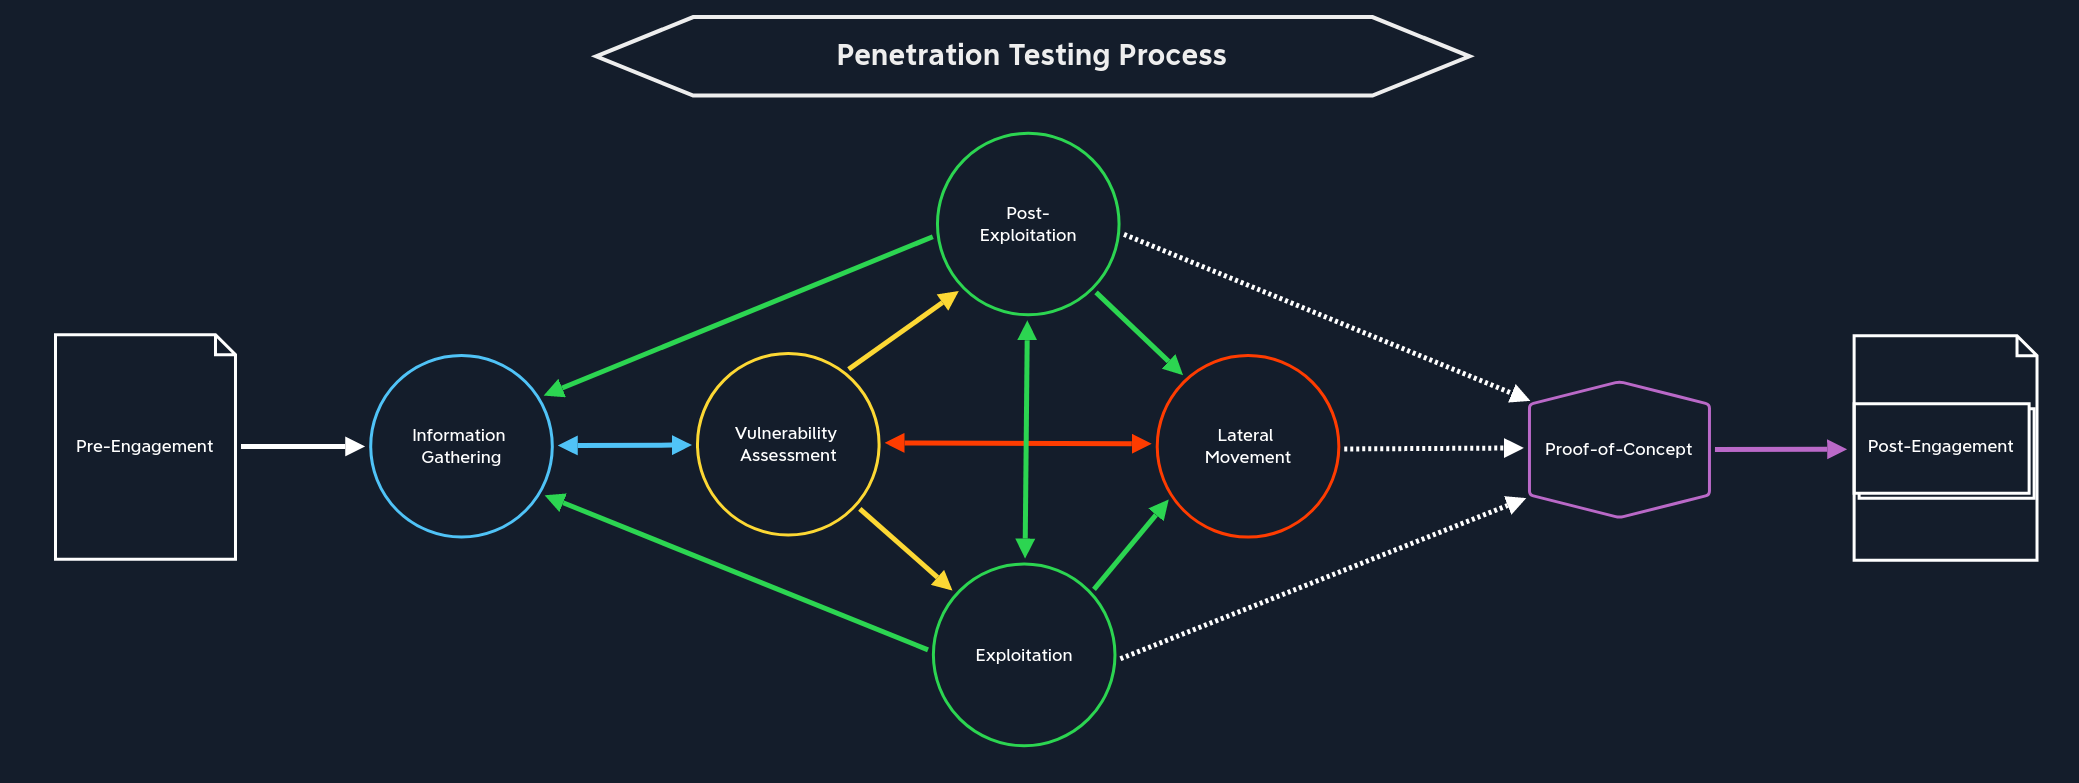
\includegraphics[width=\linewidth]{intro/process/images/post-engagement.png}
  \caption{Post-engagement}
  \label{fig:pentest-process-post-engagement}
\end{figure}

Much like there is considerable legwork before an engagement officially starts
(when testing begins), we must perform many activities (many of them
contractually binding) after our scans, exploitation, lateral movement, and
post-exploitation activities are complete. No two engagements are the same, so
these activities may differ slightly but generally must be performed to close
out an engagement fully.

\subsection{Cleanup}

Once testing is complete, we should perform any necessary cleanup, such as
deleting tools/scripts uploaded to target systems, reverting any (minor)
configuration changes we may have made, etc. We should have detailed notes of
all of our activities, making any cleanup activities easy and efficient. If we
cannot access a system where an artifact needs to be deleted, or another change
reverted, we should alert the client and list these issues in the report
appendices. Even if we can remove any uploaded files and revert changes (such
as adding a local admin account), we should document these changes in our
report appendices in case the client receives alerts that they need to follow
up on and confirm that the activity in question was part of our sanctioned
testing.

\subsection{Documentation and Reporting}

Before completing the assessment and disconnecting from the client's internal
network or sending "stop" notification emails to signal the end of testing
(meaning no more interaction with the client's hosts), we must make sure to
have adequate documentation for all findings that we plan to include in our
report. This includes command output, screenshots, a listing of affected hosts,
and anything else specific to the client environment or finding. We should also
make sure that we have retrieved all scan and log output if the client hosted a
VM in their infrastructure for an internal penetration test and any other data
that may be included as part of the report or as supplementary documentation.
We should not keep any Personal Identifiable Information (PII), potentially
incriminating info, or other sensitive data we came across throughout testing.

\subsection{Report Review Meeting}

Once the draft report is delivered, and the client has had a chance to
distribute it internally and review it in-depth, it is customary to hold a
report review meeting to walk through the assessment results. The report review
meeting typically includes the same folks from the client and the firm
performing the assessment. Depending on the types of findings, the client may
bring in additional technical subject matter experts if the finding is related
to a system or application they are responsible for. Typically we will not read
the entire report word for word but walk through each finding briefly and give
an explanation from our own perspective/experience. The client will have the
opportunity to ask questions about anything in the report, ask for
clarifications, or point out issues that need to be corrected. Often the client
will come with a list of questions about specific findings and will not want to
cover every finding in detail (such as low-risk ones).

\subsection{Deliverable Acceptance}

The Scope of Work should clearly define the acceptance of any project
deliverables. In penetration test assessments, generally, we deliver a report
marked DRAFT and give the client a chance to review and comment. Once the
client has submitted feedback (i.e., management responses, requests for
clarification/changes, additional evidence, etc.) either by email or (ideally)
during a report review meeting, we can issue them a new version of the report
marked FINAL. Some audit firms that clients may be beholden to will not accept
a penetration test report with a DRAFT designation. Other companies will not
care, but keeping a uniform approach across all customers is best.

\subsection{Post-Remediation Testing}

Most engagements include post-remediation testing as part of the project's
total cost. In this phase, we will review any documentation provided by the
client showing evidence of remediation or just a list of remediated findings.
We will need to reaccess the target environment and test each issue to ensure
it was appropriately remediated. We will issue a post-remediation report that
clearly shows the state of the environment before and after post-remediation
testing.

\subsection{Data Retention}

After a penetration test concludes, we will have a considerable amount of
client-specific data such as scan results, log output, credentials,
screenshots, and more. Data retention and destruction requirements may differ
from country to country and firm to firm, and procedures surrounding each
should be outlined clearly in the contract language of the Scope of Work and
the Rules of Engagement.

We should retain evidence for some time after the penetration test in case
questions arise about specific findings or to assist with retesting "closed"
findings after the client has performed remediation activities. Any data
retained after the assessment should be stored in a secure location owned and
controlled by the firm and encrypted at rest. All data should be wiped from
tester systems at the conclusion of an assessment. A new virtual machine
specific to the client in question should be created for any post-remediation
testing or investigation of findings related to client inquiries.

\subsection{Close Out}

Once we have delivered the final report, assisted the client with questions
regarding remediation, and performed post-remediation testing/issued a new
report, we can finally close the project. At this stage, we should ensure that
any systems used to connect to the client's systems or process data have been
wiped or destroyed and that any artifacts leftover from the engagement are
stored securely (encrypted) per our firm's policy and per contractual
obligations to our client. The final steps would be invoicing the client and
collecting payment for services rendered. Finally, it is always good to follow
up with a post-assessment client satisfaction survey so the team and
management, in particular, can see what went well during the engagement and
what could be improved upon from a company process standpoint and the
individual consultant assigned to the project. Discussions for follow-on work
may arise in the weeks or months after if the client was pleased with our work
and day-to-day interactions.

As we continually grow our technical skillset, we should always look for ways
to improve our soft skills and become more well-rounded professional
consultants. In the end, the client will usually remember interactions during
the assessment, communication, and how they were treated/valued by the firm
they engage, not the fancy exploit chain the pentester pulled off to pwn their
systems. Take this time to self-reflect and work on continuous improvement in
all aspects of your role as a professional penetration tester.

\subsection{Retired Machines}

When we have completed (at least) two modules and are satisfied with our notes
and documentation, we can select three different retired machines. These should
also differ in difficulty, but we recommend choosing two easy and one medium
machines. At the end of each module, you will find recommended retired machines
to consider that will help you practice the specific tools and topics covered
in the module. These hosts will share one or more attack vectors tied to the
module.

With the retired machines, we have a significant advantage in that we can find
existing write-ups online from many different authors (all with varying
approaches) with which we can compare our notes. If we opt to purchase a VIP
membership on the HTB main platform, we will also have access to official HTB
write-ups that present another viewpoint and often include some defensive
considerations. We can use these write-ups to compare whether we have noted
everything necessary and have not overlooked anything. The order in which we
can proceed to practice with the retired machines looks something like this:

\begin{enumerate}
    \item	Get the user flag on your own
    \item	Get the root flag on your own
    \item	Write your technical documentation
    \item	Write your non-technical documentation
    \item	Compare your notes with the official write-up (or a community write-up if you don't have a VIP subscription
    \item	Create a list of information you have missed
    \item	Watch
        \href{https://www.youtube.com/channel/UCa6eh7gCkpPo5XXUDfygQQA}{Ippsec's
        walkthrough} and compare it with your notes
    \item	Expand your notes and documentation by adding the missed parts
\end{enumerate}
